
%%%%%%%%%%%%%%%%%%%%%%% file typeinst.tex %%%%%%%%%%%%%%%%%%%%%%%%%
%
% This is the LaTeX source for the instructions to authors using
% the LaTeX document class 'llncs.cls' for contributions to
% the Lecture Notes in Computer Sciences series.
% http://www.springer.com/lncs       Springer Heidelberg 2006/05/04
%
% It may be used as a template for your own input - copy it
% to a new file with a new name and use it as the basis
% for your article.
%
% NB: the document class 'llncs' has its own and detailed documentation, see
% ftp://ftp.springer.de/data/pubftp/pub/tex/latex/llncs/latex2e/llncsdoc.pdf
%
%%%%%%%%%%%%%%%%%%%%%%%%%%%%%%%%%%%%%%%%%%%%%%%%%%%%%%%%%%%%%%%%%%%


\documentclass{article}

\usepackage[margin=1in]{geometry}
\usepackage{amssymb}
\setcounter{tocdepth}{3}
\usepackage[export]{adjustbox}
\usepackage{graphicx}
\usepackage{times}
\usepackage{hyperref}
\usepackage{cleveref}
\usepackage{wrapfig}
\usepackage{subcaption}
\crefname{subsection}{subsection}{subsections}
\usepackage{titling}
\usepackage{soul}
\usepackage{bm}
\usepackage{nicefrac}
\usepackage{xspace} % deals with the problem of when you want spaces
                    % after a macro
\usepackage[numbers]{natbib}
%\usepackage[natbibapa]{apacite}
\setcitestyle{aysep={},notesep={: }}

\newcommand{\note}[1]{\textcolor{red}{#1}}

\newif\ifcomments        % here's how we switch comments on and off
\commentstrue
   % \commentsfalse
\usepackage{our-comments} % here's where we define how we write
                          % comments to each other

% MAB: shrinking lines
%\linespread{0.971}
%\renewcommand{\topfraction}{0.9}
%\renewcommand{\bottomfraction}{0.9}
\newcommand{\defn}[1]       {{\textit{\textbf{\boldmath #1}}}}
\newcommand{\shoal}{\texttt{shoal}\xspace}
\newcommand{\Shoal}{\texttt{Shoal}\xspace}
\newcommand{\salmon}{\texttt{Salmon}\xspace}
\newcommand{\Salmon}{\texttt{Salmon}\xspace}
\newcommand{\alpine}{\texttt{alpine}\xspace}
\newcommand{\Polyester}{\texttt{Polyester}\xspace}
\newcommand{\elen}{\ensuremath{\tilde{\ell}}\xspace}
\newcommand{\tpm}{\ensuremath{\mathrm{\texttt{TPM}}}\xspace}
\newcommand{\vv}[1]{\ensuremath{\bm{#1}}\xspace}
\renewcommand{\defn}[1]       {\emph{#1}}


\newcommand{\beginsupplement}{%
        \setcounter{table}{0}
        \renewcommand{\thetable}{S\arabic{table}}%
        \setcounter{figure}{0}
        \renewcommand{\thefigure}{S\arabic{figure}}%
}


\setlength{\parskip}{5pt} % 1ex plus 0.5ex minus 0.2ex}
\setlength{\parindent}{0pt}

\begin{document}
\bibliographystyle{truncnat}




\title{{Equilibria: A Report on Comparing Resampling Methods for Robust RNA-seq Quantification Estimation}\\ \bigskip}
% \normalsize
% Avi Srivastava\textsuperscript{1},
% Micheal I. Love{2}
% Rob Patro\textsuperscript{1,}\footnote{To whom correspondence should be addressed: \href{mailto:rob.patro@cs.stonybrook.edu}{rob.patro@cs.stonybrook.edu}}\\
% \flushleft
% $^{1}$ Department of Computer Science, Stony Brook University \\}

\date{}

\maketitle
\widowpenalty=1
\clubpenalty=1

%~\citep{Glaus2012BitSeq}.
\section{Motivation}
Current research solves the problem of transcript quantification using expectation maximization based approaches.
The problem is particularly hard because of the presence of multi-mapping reads and the variance in the estimation 
of the transcript at technical, biological and inference level. Problem of multi-mapping reads due to isomorphic transcripts
are well studied by the community but the presence of variance at multiple levels drives the need to get a range estimate 
instead of point estimate per transcript in each sample without which the downstream analysis like the differential expression 
lose sensitivity and specificity.

Bootstrapping and Gibbs sampling are the most prevalent resampling methods found in RNA-seq methods literature. The former is used
before quantification optimization and resamples the reads from an equivalence class found by ~\citep{Patro2016Salmon} while latter resamples from
posterior estimates of the optimization to account for technical and inferential variance. While the current state of the art methods doesn't
specify why one should be preferred over another a recent differential expression tool (sleuth) uses bootstrap for accounting
variance in the analysis. This raises the question of what more can Gibbs sampling bring into the analysis. Currently, there is no
comparison of these resampling methods for RNA-seq quantification estimation so in this report we have compared the two resampling methods.

\section{Results}

We started with one replicate and, ran bootstrap and Gibbs sampling algorithm to get 100 samples per transcript.
First, the most intuitive way was to compare abundance values directly. So we took the mean abundance value of each transcript for both bootstrap and Gibbs sampling and visualize it through a histogram ~\cref{fig:bootGibbsHist}. Although they show good correlation with highly abundant
transcripts but there is a significant difference in the abundance values especially around 10 TPM values. ~\cref{fig:mean} derives an observation that transcript abundances below 10 TPM were of special interest since they were showing totally different frequency distribution. The observation that Bootstrap and Gibbs sample behave differently becomes even more evident with the presence of transcript on the left extreme of the scatter plot. This basically signifies that some transcripts
predicted as non-abundant by bootstrap have been given as large as 200 TPM by Gibbs Sample which needed further investigation.

\begin{figure*}
  \centering
  \begin{subfigure}[t]{0.46\textwidth}
    \centering
      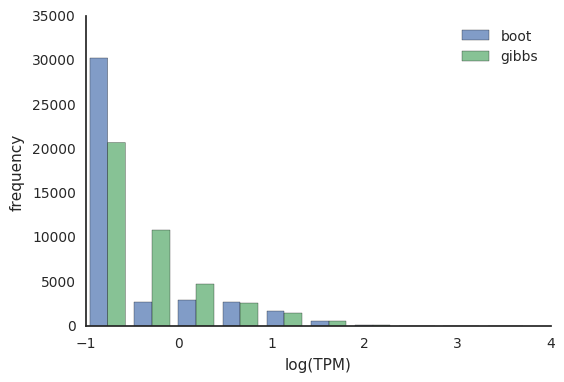
\includegraphics[width=0.9\textwidth]{figures/bootGibbsHist.png}
      \caption{\label{fig:bootGibbsHist} Histogram of abundance values (log(TPM)) for Bootstrap and Gibbs sample in one replicate.}
  \end{subfigure}
  \qquad
  \begin{subfigure}[t]{0.46\textwidth}
    \centering
    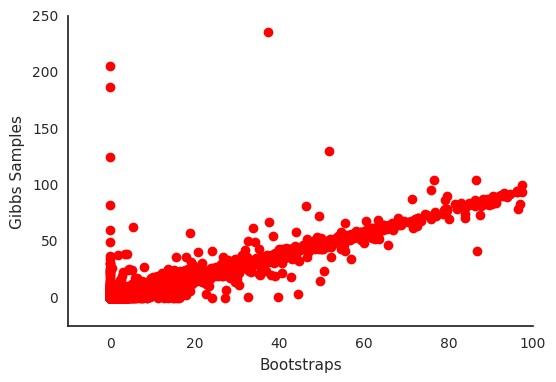
\includegraphics[width=0.9\textwidth]{figures/gibbsVBoot.png}
    \caption{ \label{fig:gibbsVBoot} Scatter plot for TPM values of Bootstrap and Gibbs Sample zoomed at 100 TPM. }
  \end{subfigure}
  \caption{Visualizing abundances in Real data}
\end{figure*}

On close observation of the transcript of interest which supposedly was `ENST00000472311' of gene `COX7A2' under RNA-seq
experiment ~\citep{kim2015comprehensive} with a COPD affected condition we found that the comparison between the posterior estimates of Bootstrap and
Gibbs Sample leads to bimodal distribution as shown in ~\cref{fig:bimodal}. On the left of the figure we see Gibbs Sample
with bimodal frequency distribution between 0 and ~200 and on the right, we have bootstrap with almost certainly all zero estimates.


\begin{figure*}
  \centering
  \begin{subfigure}[t]{0.46\textwidth}
    \centering
    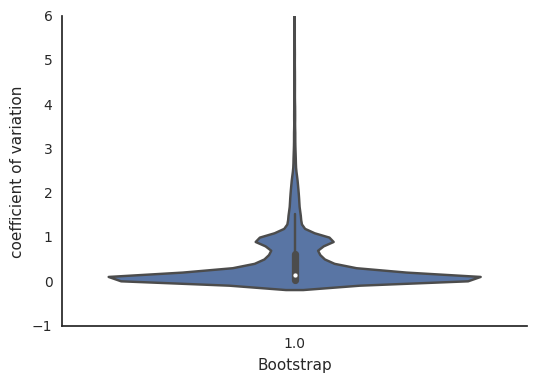
\includegraphics[width=0.9\textwidth]{figures/bootViolin.png}
    \caption{ \label{fig:bootViolin} Violin plot of coefficient of variation of all transcripts for Bootstrap in one one replicate. }
  \end{subfigure}
  \qquad
  \begin{subfigure}[t]{0.46\textwidth}
    \centering
      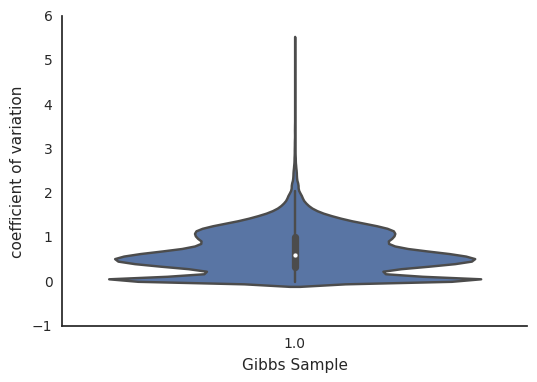
\includegraphics[width=0.9\textwidth]{figures/gibbsViolin.png}
      \caption{\label{fig:gibbsViolin} Violin plot of coefficient of variation of all transcripts for Gibbs Sample in one one replicate. }
  \end{subfigure}
  \caption{\label{fig:violin}Violin Plots on Simulated data}
\end{figure*}


To verify our findings on the real data we simulated data using polyester ~\citep{Frazee2015Polyester} and look for similar trends. In figure 
~\cref{fig:violin} we plot a violin plot for a simulated data on one of the replicates. Similar to real data we find that
plotting the violin plot for the coefficient of variation of posterior estimates of the transcripts on both the methods
gives significantly different distributions. In particular Bootstrap tends to be more conservative in assigning reads to
a transcript but with more certainty while Gibbs Sample assignment shows some variability in low abundant transcripts.


\begin{figure*}
  \centering
  \begin{subfigure}[t]{0.46\textwidth}
    \centering
    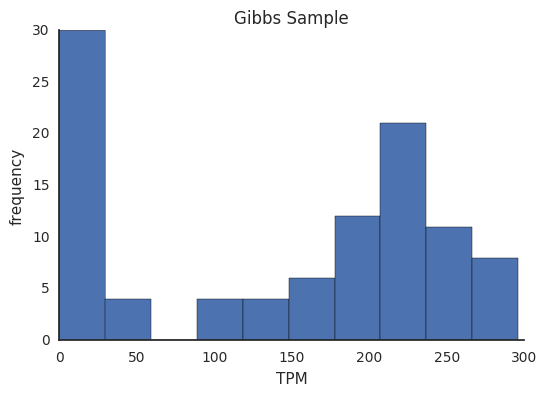
\includegraphics[width=0.9\textwidth]{figures/gibbsHist.png}
    \caption{ \label{fig:gibbsHist}Histogram of the posterior abundances of transcript `ENST00000472311' showing Bimodality in Gibbs Sampling.}
  \end{subfigure}
  \qquad
  \begin{subfigure}[t]{0.46\textwidth}
    \centering
      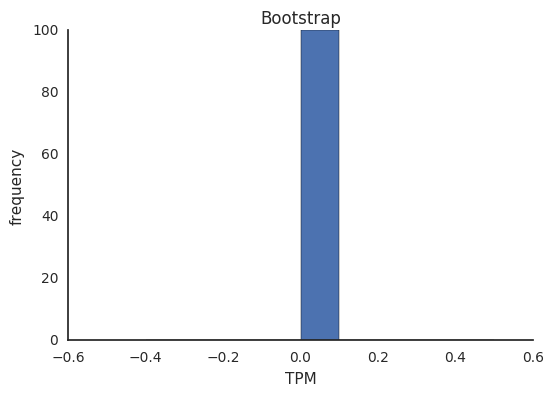
\includegraphics[width=0.9\textwidth]{figures/bootHist.png}
      \caption{\label{fig:bootHist}Histogram of the posterior abundances of transcript `ENST00000472311' in Bootstrap.}
  \end{subfigure}
  \caption{\label{fig:bimodal} Transcript level posterior abundance plot.}
\end{figure*}

 

\section{Discussion and Conclusion}


We compared two resampling methods namely, bootstrap and Gibbs Sampling and We found that estimates produced by Bootstraps tend to be more conservative while that of Gibbs sample are much more liberal and
assign low abundance to the transcript with fewer mapping. The reason being Bootstraps is more frequentist in its approach that is,
it assigns zero probability to transcripts with no mapped reads while Gibbs sample due to the availability of prior is more
bayesian in its rule and gives some probability to the transcript with no mapped read. We also observe that if a transcript
with short length gets assigned with some reads can result in a big bump in overall TPM estimates which explains the difference in
bootstrapping and Gibbs sampling procedure. Also, since there is a presence of uncertainty at multiple levels from sequencing to quantification it's not justifiable to use on/off switch on the transcript wrt abundance. we believe a more probabilistic view would be better which Gibbs Sampling in its current form ~\citep{Turro2011mmseq} provides and can be even more optimized.

One interesting future direction is since the bootstrap in its current form does not have prior information we can make bayesian
bootstrap to account for prior information. Also using uncertainty information in the form of Gibbs Sampling posterior for
differential expression analysis is another awesome!!! ;p application.



\begin{figure*}
  \centering
  \begin{subfigure}[t]{0.30\textwidth}
    \centering
    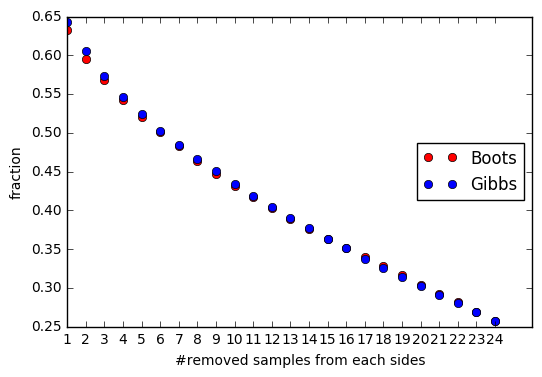
\includegraphics[width=0.9\textwidth]{figures/subsample.png}
    \caption{ \label{fig:subsample}}
  \end{subfigure}
  \qquad
  \begin{subfigure}[t]{0.30\textwidth}
    \centering
      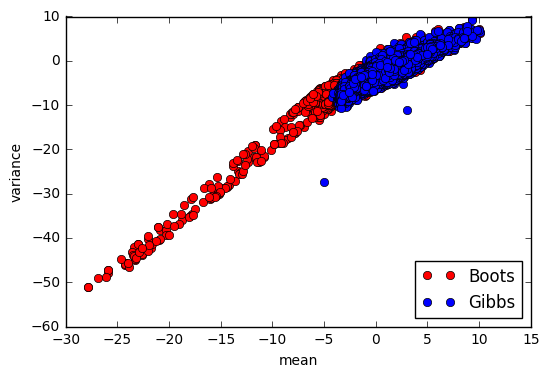
\includegraphics[width=0.9\textwidth]{figures/meanVvar.png}
      \caption{\label{fig:meanVvar}}
  \end{subfigure}
  \qquad
  \begin{subfigure}[t]{0.30\textwidth}
    \centering
      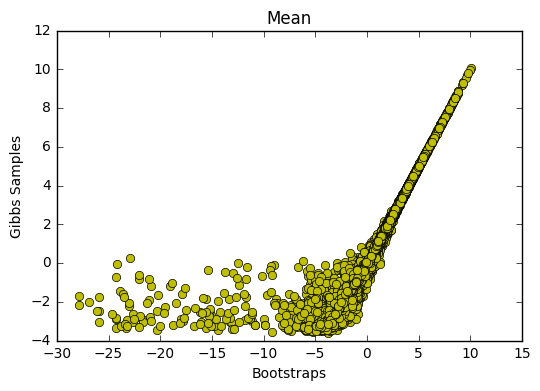
\includegraphics[width=0.9\textwidth]{figures/mean.png}
      \caption{\label{fig:mean}}
  \end{subfigure}
  \caption{Unused figures in the doc.}
\end{figure*}

\title{{Shoal: Current Progress on Empirical adaptive priors improve transcript abundance estimates in multi-sample RNA-seq data}\\ \bigskip}
\date{}

\maketitle
\widowpenalty=1
\clubpenalty=1
\setcounter{section}{0}

\section{Motivation:} Differential transcript expression is a challenging task in an RNA-seq experiment specially because of the 
presence of variance in the estimated abundances of the transcripts at multiple level in the upstream process of quantification.
Current state-of-the art quantification tools like Salmon/kallisto does an important task of quantification which is used down-stream
by the various differetianl expression analysis tools. Errors in the the differential expression analysis usually comes due to
type I errors (High False positive) and type II errors (High False Negative). 

With the decrease in the cost of Rna-Seq experiments multi-condition/multi-replicate data is readily available. The idea of using 
multi-condition data for differential expression analysis and recover from most of the type I erros with non-sginificant increase 
in the type II error has been explored deeply by many differential expression tools like Limma voom, DeSeqII. The hypothesis 
being if we imagine the empirical distribution of the abundances of the transcripts across replicates then to test for
differential expression we have compare each transcripts withing replicate distribution across multiple condition and if we 
can statistically differentiate (like t-test) between these two distribution then we can call a transcript differentially expressed.

In the above situation, typtically type I errors would be beacuse of the distributions being too far apart and our differential
expression method is able to draw a line between them to separate them. Recent differential expression tools use multi-replicate/
condition data to correct these error by shrinking. Specifically these tools works on the assumption that transcripts from one
gene would be expressed with similar abundancess across sample and shrinks the abundances towards the mean to account for errors.
Simply, in our example 


\section{Current Plan:}
\begin{itemize}
	\item Open Questions
		\begin{itemize}
			\item Isolator or any other tool in the comparison.
			\item simulation of reads is based on EM based approach, should we simulate using VBEM?
			\item learn parameter C adaptively or from multiple run of shoal.
			\item Sensitivity analysis for parameter C (MITIE would be good starting point)
		\end{itemize}
	\item Analysis
	\begin{itemize}
		\item RSEM, kallisto, MITIE, flipflop comparison
		\item Use DeSeq statistics instead of t-tests.
	\end{itemize}
	\item Writing
	\begin{itemize}
		\item No other tools have done the same thing (make it explicit).
		\item Single Sample hypothesis correction again make it explicit.
		\item TP and FN are relative, should make a comments or two.
		\item typo correction on Page3
		\item Define more about why use minimum phi in equivalence class relation.
	\end{itemize}
\end{itemize}


\bibliography{shoal}
\end{document}
